\section{Campi vettoriali}
\subsection{Definizione}
Un campo vettoriale è un'applicazione matematica formalmente indicata come 
$$
    F : \Omega \subseteq \R^n \to \R^n
$$
\underline{che associa a ogni punto  $x$ di un dato dominio uno specifico vettore $F(x)$}
\subsection{Come rappresentarli graficamente nel piano?}
Per visualizzare geometricamente un campo vettoriale nel piano bidimensionale, si utilizza una procedura che mappa i vettori sui vari punti dello spacio
\begin{enumerate}
    \item Innanzitutto, scelto un punto di coordinate $(x,y)$, si valuta la funzione per trovare il vettore corrispondente $F(x,y)$
    \item Successivamente, si trasla parallelamente questo vettore in modo che la sua origine (la "coda" della freccia) coincide esattamente con il punto $(x,y)$ di partenza
    \item Ripetendo questa operazione al variare dei punti $(x,y)$ scelti, si riempie il piano di vettori e si ottiene una rappresentazione visiva e globale del campo vettoriale
\end{enumerate}
\begin{figure}[H]
    \centering
    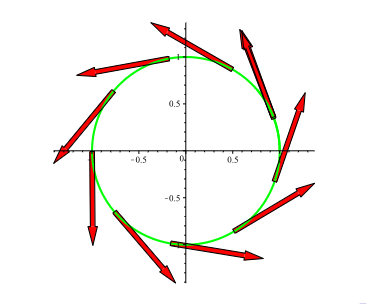
\includegraphics{figures/Schermata_20260505_113723.png}
    \label{Rappresentazione grafica del campo vettoriale di una circonferenza}
\end{figure}

\section{Integrali di linea di 2ª specie}
\subsection{Definizione}
Un integrale di linea di 2ª specie si definisce come \uline{l'integrale della componente tangenziale di un campo vettoriale $F$ lungo una curva orientata $C$}

\begin{definizione}{Formula Integrale di linea di 2ª specie}
    $$
        \int_{C} F \cdot t d\ell
    $$
    \begin{itemize}
        \item \textbf{$F$} : È il campo vettoriale su cui si opera l'integrazione
        \item \textbf{$C$} : Rappresenta la curava orientata lungo la quale si sta calcolando l'integrale
        \item \textbf{$t$} : È il versore tangente alla curva, ed è diretto secondo l'orientazione stabilita per $C$
        \item \text{d$\ell$} : Elemento differenziale di lunghezza
    \end{itemize}
\end{definizione}
\subsection{Forme differenziali e orientazione}
Gli integrali di linea di 2ª specie sono spesso scritti e calcolati utilizzando una notazione speciale chiamata
\begin{definizione}{Forma differenziale}
    $$
        \int_{C}F_{1}dx_{1}+ \cdot + F_{n}dx_{n}
    $$
    \begin{itemize}
        \item \textbf{$C$} : Rappresenta la curva orientata lungo la quale si sta calcolando l'integrale
        \item \textbf{$F_{i}$} : È la singola componente del campo vettoriale $F$
        \item \textbf{$dx_{i}$} : È il differenziale della coordinata spaziale
    \end{itemize}
\end{definizione}
Un aspetto cruciale di questi integrali risiede nel concetto di $orientazione$.

Se si calcola il lavoro svolto per andare da punto A a un punto B, e poi si calcola il lavoro svolto per percorrere la stessa curva al contrario, si otterra lo stesso numero con segno opposto
\subsection{Come calcolarli}
Per gli integrali di 2ª specie esistono 2 approcci principali
\subsubsection{Calcolo diretto tramite parametrizzazione (Metodo Standard)}
\subsection{Rappresentazione grafica}